\section{Parahoric restriction of unipotent representations}\label{sec:parahoric_restriction}

Let $G$ be a connected split simple group of simply connected type over a $p$-adic field $F$. In the previous section we stated the bijection
\begin{align*}
    \LLC^p_{\un}: G^\vee\backslash\{(x,\phi)\ |\ x\in G^\vee, \phi\in\widehat{A_x}\}\longleftrightarrow\ &\Irr_{\un}(G)\\
    (x,\phi)\hspace{1.5cm}\longmapsto \hspace{1.5cm}&(\pi_{(x,\phi)},V_{(x,\phi)}),
\end{align*}
parametrizing unipotent representations of $G$ in terms of the geometry of its complex dual group $G^\vee$. For a fixed $J\subsetneq S_{\aff}$ and corresponding parahoric subgroup $K_J$, in this section we discuss how to explicitly compute the parahoric restriction maps 
\[
    \res_{\un}^{K_J}:R_{\un}(G)\longrightarrow R_{\un}(\overline{K}_J), \quad V\longmapsto V^{U_J}
\]
from unipotent representations of $G$ to unipotent representations of $\overline{K}_J$. %The methods to explicitly compute these maps are complex and involve deep mathematics, such as the Springer correspondence or Lusztig's arithmetic-geometric correspondence. The difficulty resides in the fact that the parametrization of the unipotent representations of $p$-adic groups (given by Langlands parameters) and that of finite groups of Lie type (given by Lusztig's labels) are not related in an obvious way.
We closely follow the discussion from \cite{Reeder2000}*{\S4-8}, which we recall for convenience. However, Reeder assumes $G$ to be of adjoint type, and not all results translate as cleanly when $G$ is of simply connected type.

Let us fix throughout a unipotent representation $V=V_{(x,\phi)}$ of $G$, with $x\in G^\vee$ and $\phi\in\widehat{A_x}$. 
%We want to decompose the $\overline{K}_J$-module $V^{U_J}$ as a direct sum of irreducible submodules. More concretely, 
For each irreducible unipotent $\overline{K}_J$-representation $\chi$, we want to calculate the value of 
$\langle\chi,V^{U_J}\rangle_{K_J},$
where we view the $\overline{K}_J$-representations as $K_J$-representations trivial on $U_J$.

In the first part, we state two reduction steps that allow us to reduce the problem of calculating the parahoric restrictions of $V$ to the problem of calculating the restriction of some representation obtained from $V$ over a reflection group with respect to certain reflection subgroups. This part does not require $G$ to be of adjoint type. For example, if $V$ is Iwahori-spherical, we obtain a representation $V^{\mathbf{1}}_{q=1}$ over the affine Weyl group $W_{\aff}=W\ltimes X(T^\vee)$ of $G$, and the parahoric restriction of $V$ can be determined by studying the representation $V^{\mathbf{1}}_{q=1}|_{\widetilde{W}_J}$ where $\widetilde{W}_J$ is the subgroup of $W_{\aff}$ generated by the reflections in $J$. Springer theory is then the key theoretical tool that allows us to calculate the action of $W_{\aff}$ on $V^{\mathbf{1}}_{q=1}$. We devote the second part of the chapter to discuss this. However, not every unipotent representation of $G$ is Iwahori-spherical, so in the last part we discuss a more general method to calculate the parahoric restriction of non Iwahori-spherical representations with the use of weight diagrams developed in \cite{Reeder1997}. These have been computed for all unipotent representations of adjoint exceptional groups in \cite{Reeder2000}*{\S 9}.

\subsection{Reduction to representations over reflection groups}

Consider the fixed unipotent representation $V=V_{(x,\phi)}$ of the simply connected $p$-adic group $G$. By Corollary \ref{cor:unipotentblock_disjoint}, there is a unique proper subset $I$ of $S_{\aff}$ with corresponding standard parahoric $K:=K_I$, such that $V^{U_K}$ contains a cuspidal unipotent representation $\sigma$ of $\overline{K}$. In particular, the vector space 
\begin{equation}\label{eqn:Vsigma}
    V^\sigma:=\Hom_K(\sigma,V^{U_K})=\Hom_K(\sigma,V)=\Hom_G(\cInd_K^G\sigma,V)    
\end{equation}
is a non-zero irreducible $\cH(G,K,\sigma)=\End_G(\cInd_K^G\sigma)$-module. The passage $V\mapsto V^\sigma$ is known to lose no information about the representation $V$ (\cite{BushnellKutzko1998},\cite{Lusztig1995}). %We say that the block parametrized by the pair $(K,\sigma)$ is controlled by the Hecke algebra $\cH(G,K,\sigma)$. 

Similarly, if $\chi$ is an irreducible unipotent representation of $\overline{K}_J$, there is a unique proper subset $I'$ of $S_{\aff}$ contained in $J$ such that $\chi$ is a subrepresentation of $\Ind_{K_{I'}}^{K_J}\sigma'$, where $\sigma'$ is a cuspidal unipotent representation of $\overline{K}_{I'}$. In particular, the vector space
$$\chi^{\sigma'}:=\Hom_{K_{I'}}(\sigma',\chi)=\Hom_{K_J}(\Ind_{K_{I'}}^{K_J}\sigma',\chi)\neq0$$
is naturally a $\cH(K_J,K_{I'},\sigma')$-module, where $\cH(K_J,K_{I'},\sigma')\cong\End_{K_J}(\Ind_{K_{I'}}^{K_J}\sigma')$ is the subalgebra of functions of $\cH(G,K_{I'},\sigma')$ supported on $K_J$.

\begin{lemma}[First reduction]\label{lem:multiplicity} (\cite{Reeder2000}*{\S 4.2})
    The multiplicity of the simple $K_J$-module $\chi$ in $V^{U_J}$ is given by 
    $$\langle\chi,V^{U_J}\rangle_{K_J}=\langle\chi^{\sigma'},V^{\sigma'}\rangle_{\cH(K_J,K_{I'},\sigma')}.$$
    Moreover, $\langle\chi,V^{U_J}\rangle=0$ unless $I=I'$. In particular, if $J$ does not contain $I$, then $V^{U_J}=0$.
\end{lemma}
\begin{proof}
    Since $U_J\subseteq U_{I'}$, we have that
    \begin{align*}
        V^{\sigma'}=\Hom_{K_{I'}}(\sigma',V)&=\Hom_{K_{I'}}(\sigma',V^{U_J})\simeq\Hom_{K_J}(\Ind_{K_{I'}}^{K_J}\sigma',V^{U_J})\\
        &\simeq\bigoplus_\eta\langle\eta,V^{U_J}\rangle_{K_J}\Hom_{K_J}(\Ind_{K_{I'}}^{K_J}\sigma',\eta)\\
        &\simeq\bigoplus_\eta\langle\eta,V^{U_J}\rangle_{K_J}\eta^{\sigma'},
    \end{align*}
    and therefore
    \begin{equation*}
        \langle\chi^{\sigma'},V^{\sigma'}\rangle_{\cH(K_J,K_{I'},\sigma')}=\sum_\eta\langle\chi^{\sigma'},\eta^{\sigma'}\rangle_{\cH(K_J,K_{I'},\sigma')}\langle\eta,V^{U_J}\rangle_{K_J}=\langle\chi,V^{U_J}\rangle_{K_J}.
    \end{equation*}
    To prove the second statement, we note that $V^{\sigma'}\neq0$ if and only if $(K,\sigma)=(K_{I'},\sigma')$ by Corollary \ref{cor:unipotentblock_disjoint}. In other words, $I=I'$ and the last assertion follows immediately from the fact that $J$ contains $I'$.
\end{proof}

\begin{example}
    Let us briefly explore the two extreme cases of the above result.
    \begin{itemize}
        \item If $V$ is a Iwahori-spherical representation of $G$, then $V^{\cI}\neq 0$, $I=\emptyset$ and the pair $(K,\sigma)$ is given by $(\cI,\mathbf{1})$. In this case, Lemma \ref{lem:multiplicity} states that 
        $$\langle\chi,V^{U_J}\rangle_{K_J}=\langle\chi^\cI,V^\cI\rangle_{\cH(K_J,\cI,\mathbf{1})}.$$
        Thus, $V$ has a non-zero parahoric restriction for any $J\subsetneq S_{\aff}$.
        \item If $V$ is a supercuspidal unipotent representation of $G$, then $I$ is a maximal proper subset of $S_{\aff}$ and $V^{U_J}=0$ unless $J=I$.
    \end{itemize}
\end{example}

For the second reduction step we consider $R=\CC(v,v^{-1})$, where $v$ is an indeterminate and define $\cH(G,K,\sigma)_v$ to be the \textit{generic Hecke algebra} defined over $R$ with the same generators and relations as $\cH(G,K,\sigma)$, but with $q$ replaced by $v^2$ in the quadratic relations. By specializing this generic Hecke algebra we recover
$$\cH(G,K,\sigma)_{\sqrt{q}}=\cH(G,K,\sigma),\quad\quad \cH(G,K,\sigma)_1=\CC[\tilde{W}(K,\sigma)],$$
where $\tilde{W}(K,\sigma)$ is an explicit affine reflection group associated to the pair $(K,\sigma)$ (see \cite{Lusztig1995} for an explicit list, and \cite{Carter1985}*{\S10} for a detailed construction). When $K=\mathcal{I}$ is the Iwahori subgroup and $\sigma=\mathbf{1}$ is the trivial representation, $\mathcal{H}(G,\mathcal{I},\mathbf{1})_1=\CC[\widetilde{W}]$, where $\widetilde{W}$ is the affine Weyl group. Instead, if $K$ is a maximal parahoric subgroup of $G$, then $\cH(G,K,\sigma)\cong\CC$ so $\tilde{W}(K,\sigma)$ is trivial.

\textbf{Fact:} For any simple $\cH(G,K,\sigma)$-module $E$ \textit{considered in this document}, there is a $\cH(G,K,\sigma)_v$-module $E_v$ such that 
\[
    E\simeq E_v\otimes_R\CC, \text{ where }f\in R\text{ acts on $\CC$ by }f(\sqrt{q}).
\]
It then follows that we have a $q=1$ operation that takes modules over Hecke algebras to modules over the corresponding reflection groups, obtained by setting $v=1$ in all matrix coefficients of the generic module.

\begin{proposition}[Second reduction]\label{prop:second_red}(\cite{Reeder2000}*{\S6.1})
    Let $J\subsetneq S_{\aff}$ and let $(K,U_K,\overline{K})$ be a parahoric subgroup contained in $(K_J,U_J,\overline{K}_J)$ with cuspidal unipotent $\overline{K}$-representation $\sigma$. Then the diagram 
    \[
        \begin{tikzcd}
        \cH(G,K,\sigma)\textrm{-mod} \arrow[r, "q=1"] \arrow[d, "\Res_{\cH(K_J,K,\sigma)}"'] & \tilde{W}(K,\sigma)\textrm{-mod} \arrow[d, "\Res_{\tilde{W}(K,\sigma)_J}"] \\
        \cH(K_J,K,\sigma)\textrm{-mod} \arrow[r, "q=1"] & \tilde{W}(K,\sigma)_J\textrm{-mod}
        \end{tikzcd}
    \]
    is commutative, and the bottom arrow is an isometry with respect to the usual inner product of character. That is, for any irreducible $K_J$-module $\chi$, we have that 
    \begin{equation}
        \langle\chi^\sigma,V^\sigma\rangle_{\cH(K_J,K,\sigma)}=\langle\chi^\sigma_{q=1},V^\sigma_{q=1}\rangle_{\tilde{W}(K,\sigma)_J}.
    \end{equation}
\end{proposition}

Combining both reduction steps, we obtain the identity
\begin{equation}\label{eqn:reduction_steps}
    \langle\chi,V^{U_J}\rangle_{K_J}=\langle\chi^\sigma,V^\sigma\rangle_{\mathcal{H}(K_J,K,\sigma)}=\langle\chi^\sigma_{q=1},V^\sigma_{q=1}\rangle_{\tilde{W}(K,\sigma)_J}
\end{equation}
Thus, to compute the parahoric restriction $V^{U_J}$, it suffices to study the $\tilde{W}(K,\sigma)_J$-module $V_{q=1}^\sigma$. By calculating its decomposition into $\tilde{W}(K,\sigma)$-irreducible representation, one can directly obtain the decomposition of $V^{U_J}$ into irreducible $\overline{K}_J$-representations. 

At this point, we restrict our attention to the parahoric restriction of Iwahori-spherical representations, for Springer theory provides a way to calculate the $\tilde{W}(I,\mathbf{1})_J$-module $V^\mathbf{1}_{q=1}$ explicitly, differing significantly from the non Iwahori-spherical case. As stated above, for Iwahori-spherical representations, the reflection subgroup $\tilde{W}(\cI,\mathbf{1})\cong W_{\aff}$ is simply the affine Weyl group of $G$, and $\tilde{W}(\cI,\mathbf{1})_J=\widetilde{W}_J$ is the subgroup of $\widetilde{W}$ generated by the simple reflections of the roots in $J$.

\subsection{The Iwahori-spherical case and the Springer correspondence}\label{subsec:Iwahori_spherical}

Given an Iwahori-spherical representation $V=V_{(x,\phi)}$ of $G$ and a proper subset $J\subsetneq S_{\aff}$, in the previous subsection we proved that  
\begin{equation}\label{eqn:multiplicity_Iwahori}
    \langle\chi,V^{U_J}\rangle_{\overline{K}_J}=\langle\chi^\mathbf{1}_{q=1},V^\mathbf{1}_{q=1}\rangle_{\widetilde{W}_J}.
\end{equation}
for any principal series representation $\chi$ of the reductive quotient $\overline{K}_J$. To extract describe the structure of the $\widetilde{W}_J$-module $V^\mathbf{1}_{q=1}$ in terms of the geometry of the dual group and the data $(x,\phi)$, Springer theory provides a powerful tool. Let $x=us$ be the Jordan decomposition of $x$, with $u\in G^\vee$ unipotent and $s\in G^\vee$ semisimple. By conjugating if necessary, we assume that $s\in T^\vee$ for a fixed split maximal torus of $G^\vee$. Let $\mathcal{B}$ and $\mathcal{B}_s$ be the flag varieties of the complex reductive groups $G^\vee$ and $M^\vee:=Z_{G^\vee}(s)^0$, respectively, and consider the Springer fibres $\mathcal{B}^x$ and $\mathcal{B}_s^u$ parametrizing the set of Borel subgroups of $G^\vee$ containing $x$ and the set of Borel subgroups of $M^\vee$ containing $u$. Let $W_M$ be the Weyl group of $M^\vee$, isomorphic to the subgroup of $W$ generated by all reflections of roots trivial on $s$.

While the varieties $\mathcal{B}_x$ and $\mathcal{B}_s^u$ do not admit a natural action of $W$ and $W_M$, respectively, Lusztig showed using the theory of perverse sheaves that the singular cohomology spaces $H^*(\mathcal{B}_x)$ and $H^*(\mathcal{B}_s^u)$ do. The $W_M$ structure of $H^*(\mathcal{B}_s^u)$ can be easily read from the Springer correspondence for the reductive group $M^\vee$ via the Green tables, which are well understood. Moreover, the module structures are tightly related by the formula (\cite{Kato1983}*{Proposition 2.5}),
$$H^*(\mathcal{B}^x)\cong\Ind_{W_M}^W H^*(\mathcal{B}_s^u).$$
Kato also showed that this action could naturally be extended to an action of the affine Weyl group $W_{\aff}=W\ltimes X(T^\vee)$, where $X=X(T^\vee)$ is the character lattice of $T^\vee$. The semisimple element $s\in T^\vee$ is naturally a character of $X$ given by evaluation. Thus, the cohomology spaces $H^*(\mathcal{B}^x)$ carry a natural $W_{\aff}$-action given by 
$$H^*(\mathcal{B}^x)=\Ind_{W_{M,\aff}}^{W_{\aff}} H^*(\mathcal{B}_s^u)\otimes s,$$
where $W_{M,\aff}=W_M\ltimes X$ (see \cite{Kato1983}*{Proposition 3.2}).

Finally, the component group $A_x$ acts naturally on the varieties $\mathcal{B}^x$ and $\mathcal{B}^u_s$ by conjugation, inducing a natural action on the cohomology spaces $H^*(\mathcal{B}^x)$ and $H^*(\mathcal{B}_s^u)$. While the $A_x$-action on $H^*(\mathcal{B}^x)$ commutes with the $W_{\aff}$-action, thus giving an $A_x\times W_{\aff}$-module structure, the $A_x$-action on $H^*(\mathcal{B}_s^u)$ does not necessarily commute with the $W_{M,\aff}$-action. The precise structure of this action is subtle, and we closely follow the discussion in \cite{Kato1983}*{\S 6} to explain this.

Given $x=su$ as above, let $W_s$ be the stabilizer of $s$ in $W$. Then $W_M$ is a normal subgroup of $W_s$, and the quotient is the component group of the centralizer of $s$ in $G^\vee$:
$$W_s/W_M\cong Z_{G^\vee}(s)/Z_{G^\vee}(s)^0\cong R=\{w\in W_s\ |\ w(\Delta_M^+)=\Delta_M^+\}.$$
By choosing Kac coordinates for $s$, the group $R$ can be seen as a subgroup of the fundamental group $\Omega$, and in addition it normalizes $W_M$ so $W_s=W_M\rtimes R$. Moreover, Kato defines the canonical subgroup 
$$R(u)=\{w\in R\ |\ u^{n(w)}\text{ and $u$ are conjugate in $M^\vee$}\}.$$
Since $Z_{G^\vee}(x)=Z_{G^\vee}(s)\cap Z_{G^\vee}(u)$, we have that $Z_{M^\vee}(u)\triangleleft Z_{G^\vee}(x)$ and $Z_{G^\vee}(x)/Z_{M^\vee}(u)\cong R(u)$. In particular, we may regard $A^{M^\vee}_u:=Z_{M^\vee}(u)/Z_{M^\vee}(u)^0$ as a normal subgroup of $A_x$, and we have the isomorphism $A_x/A^{M^\vee}_u\cong R(u)$. 

Denote by $j:Z_{G^\vee}(s)\rightarrow R$ the canonical surjection and note that each $y\in Z_{G^\vee}(x)\leq Z_{G^\vee}(s)$ defines a map $H^i(\mathcal{B}_s^u)\rightarrow H^i(\mathcal{B}_s^u)$, which we also denote by $y$. Moreover, for each $w\in W_{M,\aff}$, it follows from the definitions of the $W_{M,\aff}$ that \cite{Kato1983}*{(6.1)}
$$y\cdot w=\prescript{j(y)}{}{w}\cdot y:H^i(\mathcal{B}_s^u)\longrightarrow H^i(\mathcal{B}_s^u).$$
With this in mind, we consider the induced surjection $j_0:A_x\rightarrow R(u)$ and, since $R(u)$ acts on $W_{M,\aff}$ by conjugation, we can construct the semidirect product $A_x\ltimes W_{M,\aff}$. This group embeds in $A_x\times W_{\aff}$ via the map $(a,w)\mapsto(a,j_0(a)w)$ (the image in fact lands inside $A_x\times W_{s,\aff}$), and Kato shows that the $A_x$-action on $H^*(\mathcal{B}_s^u)$ extends to an $A_x\ltimes W_{M,\aff}$-action. In particular, we have the following result.

\begin{proposition}[\cite{Kato1983}*{Proposition 6.2}]
    As $A_x\times W_{\aff}$-modules, we have
    $$H^*(\mathcal{B}^x)\cong\Ind_{A_x\ltimes W_{M,\aff}}^{A_x\times W_{\aff}} H^*(\mathcal{B}_s^u).$$
\end{proposition}
Let us now go back to representations of $p$-adic groups. Let $V_{(x,\phi)}$ be an Iwahori-spherical unipotent representation of $G$. Then $V_{(x,\phi)}^\mathcal{I}$ is a simple $\mathcal{H}(G,\mathcal{I},\mathbf{1})$-module, while $V_{(x,\phi),q=1}^\mathbf{1}$ is a simple $W_{\aff}$-module. We then have the following central result, due to Lusztig. We remark that up to this point we have not used the fact that $G$ is of simply connected type, so this result holds more generally by swapping $W_{\aff}$ with an adequate subgroup of the extended affine Weyl group $\widetilde{W}$.

\begin{theorem}\label{thm:Kato_module}\cite{Lusztig1995b}
    Let $V_{x,\phi}$ be an Iwahori-spherical irreducible representation of $G$. After letting $q\rightarrow 1$ and then taking semisimplification, the simple $\mathcal{H}(G,I,\mathbf{1})$-module $V^\mathbf{1}_{x,\phi}$ becomes the $W_{\aff}$-module $\varepsilon\otimes H^*(\mathcal{B}^x)^\phi$, where $\varepsilon$ is the sign representation of $W_{\aff}$.
\end{theorem}

\begin{remark}\label{rem:Weylgroups}
    An important remark is due at this point. The above theorem relates the structure of $V^\mathbf{1}_{(x,\phi),q=1}$ with the structure of $H^*(\mathcal{B}^x)^\phi$ as $W_{\aff}$-modules. However, the former object is naturally $p$-adic, while the latter is complex analytic. The Weyl groups of $G$ and $G^\vee$ are canonically isomorphic, but not equal if the group is not simply laced, since the isomorphism swaps short with long roots. It is a standard abuse of notation to denote both Weyl groups with the same symbol, but one needs to be careful during explicit calculations inside which Weyl group one is working. We are ultimately interested in the $p$-adic side, but most computations involving cohomology groups and the Springer correspondence take place in the complex side. In particular, the reflection $s_0$ inside $W$ will be a \textbf{short} reflection, corresponding to the highest short root. At the very end, we then trace the representations back to the $p$-adic side by swapping long and short roots. 
\end{remark}

Let us discuss some consequences of Theorem \ref{thm:Kato_module}. When $R(u)=\{1\}$, the semidirect product $A_x\ltimes W_{M,\aff}$ is simply the direct product $A_x\times W_{M,\aff}$, and we have that 
\begin{equation}\label{eqn:Kato_isotropic}
    H^*(\mathcal{B}^x)^\phi=\left(\Ind_{A_x\times W_{M,\aff}}^{A_x\times W_{\aff}}H^*(\mathcal{B}_s^u)\right)^\phi=\Ind_{W_{M,\aff}}^{W_{\aff}}H^*(\mathcal{B}_s^u)^\phi.
\end{equation}
From \eqref{eqn:multiplicity_Iwahori} and Theorem \ref{thm:Kato_module}, the computation of the parahoric restriction of $V_{(x,\phi)}$ is then reduced to the computation of the $\widetilde{W}_J$-module structure of $H^*(\mathcal{B}^x)^\phi$. The difficulty of this case comes from simultaneously controlling the action of the character lattice $X$ on $H^*(\mathcal{B}_s^u)^\phi$. In \cite{Reeder2000}, Reeder observes that the canonical projection from $W_{\aff}$ to $W$ is injective on each $\widetilde{W}_J$ with image $W_J$. If $\psi_J:W_J\rightarrow \widetilde{W}_J$ is the inverse of this map, then we can consider the pullback $\psi_J^*$ of representations of $\widetilde{W}_J$ to representations of $W_J$. By \eqref{eqn:Kato_isotropic} and Mackey theory, we have that 

\begin{equation}\label{eqn:mackey_generalcase}
    \psi_J^*\left[\left(\Ind_{\widetilde{W}_M}^{\widetilde{W}}H^*(\mathcal{B}^u_s)^\phi\right)|_{\widetilde{W}_J}\right]\cong\bigoplus_{w\in W_M\backslash W/W_J}\Ind_{W_{J,s^w}}^{W_J}\chi_{s^w}^J\otimes\left[H^*(\mathcal{B}^u_s)^\phi\right]^w,
\end{equation}

where $W_{J,s^w}=W_M^w\cap W_J$ and $\chi_{s^w}^J=\chi_{s^w}\circ\chi_J:W_{J,s^w}\rightarrow \mathbb{C}^\times$. To use this formula we need an understanding of the groups $W_{J,s^w}$ and the characters $\chi_{s^w}^J$. The groups $W_{J,t}$ have been studied in the literature, and they can be decomposed into 
$$W_{J,t}=W_{J,t}^0\rtimes R_{J,t},$$
where $W_{J,t}^0$ is a ``large" reflection subgroup of $W$ generated by the reflections in $J$ that fix $t$, and $R_{J,t}$ is a ``small'' group that normalizes $W_{J,t}^0$. The character $\chi_t^J$ is trivial on $W_{J,t}^0$ and is determined by its restriction to $R_{J,t}$. As a result, the characters $\chi_t^J$ are trivial in many cases. 
%For example, if $W_{J,t}=W_{J,t}^0$ is a reflection subgroup of $W$, then $\chi_t^J$ is trivial.
%In addition, one can associate to $J$ a subgroup $Z_J$ of the center of the simply connected cover of the pseudo-Levi subgroup $G^\vee_J$ generated by the torus and the roots $J$, and if the order of $s$ is relatively prime to the order of $Z_J$, then $\chi_s^J$ is trivial as well (\cite{Reeder2000}*{Lemma 8.3}). 
We refer to \cite{Reeder2000}*{\S 8} for a detailed discussion on the structure of these characters, where explicit formulas to compute them are provided. If all characters $\chi_{s^w}^{J}$ appearing in \eqref{eqn:mackey_generalcase} are trivial, then computations are greatly simplified.
\begin{lemma}\label{lem:mackey_restriction}
    With the same notation as in \eqref{eqn:mackey_generalcase}, if the characters $\chi_{s^w}^{J}$ are trivial for all $w\in W_s\backslash W/W_J$, then
    $$\psi_J^*\left[\left(\Ind_{\widetilde{W}_s}^{\widetilde{W}}H^*(\mathcal{B}^u_s)^\phi\right)|_{\widetilde{W}_J}\right]\cong\left(\Ind_{W_s}^W H^*(\mathcal{B}^u_s)^\phi\right)|_{W_J}$$
\end{lemma}
\begin{proof}
    This is an immediate consequence of Mackey's formula applied to the right hand side of \eqref{eqn:mackey_generalcase}.
\end{proof}



Since the $p$-adic group $G$ is simply connected, maximal parahoric subgroups of $G$ are in bijection with the maximal proper subsets of $S_{\aff}$. In addition, the extended affine Dynkin diagram $S_{\aff}$ has a natural $\Omega$-action, where $\Omega$ is the fundamental group of the adjoint group $G_{\ad}$. Any non-trivial $\omega\in\Omega$ induces an inner automorphism of $G_{\ad}$ but an outer automorphism of $G$, which we also denote by $\omega$. Fix some maximal subset $J\subsetneq S_{\aff}$ and let $J'=\omega(J)$. While the parahoric restrictions with respect to $K_J$ and $K_{J'}=\omega(K_J)$ are not always isomorphic as $\overline{K}_J$- and $\overline{K}_{J'}=\omega(\overline{K}_J)$-modules, one can be deduced from the other. The main idea is that the corresponding maximal parahoric subgroups $K_J$ and $K_{J'}$ are conjugate in $G_{\ad}$ since $\omega$ is an inner automorphism. One can then relate parahoric restrictions of representations of $G_{\ad}$ with representations of $G$.

More concretely, let $x=su$ be the Jordan decomposition of $x\in G^\vee$. Let $\tilde{u}$ be the unique unipotent lift of $u$ in the simply connected cover $G_{\scn}^\vee$ of $G^\vee$ and fix any lift $\tilde{s}$ of $s$ in $G_{\scn}^\vee$. Then $\tilde{x}=\tilde{s}\tilde{u}$ is a lift of $x$ in $G_{\scn}^\vee$. Since $\tilde{u}$ is the unique unipotent lift of $u$, the canonical map $Z_{G_{\scn}^\vee}(\tilde{u})\rightarrow Z_{G^\vee}(u)$ is surjective. While the map $Z_{G_{\scn}^\vee}(\tilde{s})\rightarrow M^\vee:=Z_{G^\vee}(s)^0$ is well-defined and surjective, the group $Z_{G^\vee}(s)$ may be disconnected, with component group isomorphic to $R$. Consider now the composition
$$Z_{G_{\scn}^\vee}(\tilde{x})=Z_{Z_{G_{\scn}^\vee}(\tilde{s})}(\tilde{u})\twoheadrightarrow Z_{M^\vee}(u)\hookrightarrow Z_{Z_{G^\vee}(s)}(u)=Z_{G^\vee}(x).$$
The first map is surjective (follows from the above observation) while the second map is clearly injective.
Since $Z_{G^\vee}(s)/M^\vee\cong R$, we have that $Z_{G^\vee}(x)/Z_{M^\vee}(u)\cong R(u)$ by definition. Recall that $A_{\tilde{x}}$ and $A_x$ are the component groups of $Z_{G_{\scn}^\vee}(\tilde{x})$ and $Z_{G^\vee}(x)$, respectively, and let $A_x^0$ be the component group of $Z_{M^\vee}(u)$. It then follows that $A_x\cong A_x^0\rtimes R(u)$, and we have the short exact sequence 
\begin{equation}\label{eqn:SES_comp}
    1\rightarrow Z/(Z\cap Z_{G_{\scn}^\vee}(\tilde{x})^0)\rightarrow A_{\tilde{x}}\rightarrow A_x^0\rightarrow 1,
\end{equation}
which implies that there is a bijection $\phi\leftrightarrow\tilde{\phi}$ between irreducible representations of $A_x^0$ and irreducible representations of $A_{\tilde{x}}$ trivial on the centre $Z$. Following an analogous construction, the pair $(\tilde{x},\tilde{\phi})$ gives rise to an irreducible $\widetilde{W}$-module $H^*(\mathcal{B}^{\tilde{x}})^{\tilde{\phi}}$ satisfying that 
$$H^*(\mathcal{B}^{\tilde{x}})^{\tilde{\phi}}|_{W_{\aff}\rtimes R(u)}\cong H^*(\mathcal{B}^x)^\phi,$$
where $R(u)$ is naturally seen as a subgroup of $\Omega$.
Each character $\chi$ of $R(u)$ then can be inflated to a character of $A_x\cong A_x^0\rtimes R(u)$ giving a final decomposition into irreducible $W_{\aff}$-modules
$$H^*(\mathcal{B}^{\tilde{x}})^{\tilde{\phi}}|_{W_{\aff}}\cong\bigoplus_{\chi\in\widehat{R(u)}} H^*(\mathcal{B}^x)^{\phi\otimes\chi}.$$

Let us now consider the two extreme cases of the above discussion. On one hand, if $R(u)=\{1\}$, then $Z_{G_{\scn}^\vee}(\tilde{x})\rightarrow Z_{G^\vee}(x)$ is surjective and $A_x=A_x^0$. Thus, it follows that 
\begin{equation}\label{eqn:isom_cover}
    H^*(\mathcal{B}^{\tilde{x}})^{\tilde{\phi}}|_{W_{\aff}}\cong H^*(\mathcal{B}^x)^\phi
\end{equation}
as $W_{\aff}$-modules. Since $H^*(\mathcal{B}^x)^\phi$ is obtained as the restriction of an irreducible $\widetilde{W}$-module and $\omega\in\widetilde{W}$ it then follows that for any $J\subsetneq S_{\aff}$,
\begin{equation}\label{eqn:twist_Ru_trivial}
    H^*(\mathcal{B}^x)^\phi|_{\widetilde{W}_J}\cong (H^*(\mathcal{B}^x)^\phi|_{\widetilde{W}_{\omega(J)}})^\omega
\end{equation}
as $\widetilde{W}_J$-modules.

On the other hand, if $R(u)=\Omega$, then 
$$H^*(\mathcal{B}^{\tilde{x}})^{\tilde{\phi}}|_{W_{\aff}}\cong\bigoplus_{\chi\in\widehat\Omega} H^*(\mathcal{B}^x)^{\phi\otimes\chi}$$
as irreducible $W_{\aff}$-modules and standard Clifford theory states that the action of $\Omega$ permutes these components transitively. In particular, this means that for any $J\subsetneq S_{\aff}$ and $\omega\in\Omega\subset\widetilde{W}$ there is some character $\tau\in\widehat{\Omega}$ such that for all characters $\chi\in\widehat{\Omega}$, 
\begin{equation}\label{eqn:twist_Ru_nontrivial}
    H^*(\mathcal{B}^x)^{\phi\otimes\chi}|_{\widetilde{W}_J}\cong (H^*(\mathcal{B}^x)^{\phi\otimes\chi\tau}|_{\widetilde{W}_{\omega(J)}})^\omega.
\end{equation}

We have thus shown

\begin{proposition}\label{prop:twist_fund_group}
    Let $V_{(x,\phi)}$ be an Iwahori-spherical representation of $G$, of simply connected type. Fix some $J\subsetneq S_{\aff}$ and $\omega\in\Omega$, which induces an isomorphism of reductive quotients $\omega:\overline{K}_J\cong\overline{K}_{\omega(J)}$. Then $V_{(x,\phi)}^{U_J}$ is isomorphic to $V_{(x,\phi\otimes\tau)}^{U_{\omega(J)}}$ as $\overline{K}_J$-modules via $\omega$ for some character $\tau$ of $R(u)$ lifted to $A_x$ and is independent of $\phi$. In particular, if $R(u)=\{1\}$, then $V_{(x,\phi)}^{U_J}$ and $V_{(x,\phi)}^{U_{\omega(J)}}$ are isomorphic as $\overline{K}_J$-modules.
\end{proposition}

If $G$ is a group of exceptional type, then the above result covers all possible cases, for $\Omega$ is either trivial or has orders $2$ or $3$. We encourage the reader to check Table \ref{tbl:E6_hyperspecialWJ0}, where this result can be clearly observed.

\newpage











\iffalse
The Springer correspondence explicitly describes the action of the Weyl group on the top cohomology group.

\begin{theorem}
    Let $G^\vee$ be a complex algebraic reductive group with Weyl group $W$. For each pair $(u,\phi)$, where $u\in G^\vee$ is a unipotent element and $\phi$ is an irreducible character of $A_u$, the $\phi$-isotropic subspace of the top cohomology group $H^{\mathrm{top}}(\mathcal{B}^u)^\phi$ is either zero or an irreducible $W$-representation. Moreover, each irreducible character of $W$ arises this way for exactly one pair $(u,\phi)$ up to $G^\vee$ conjugation. In other words, there is an injection
    $$\Irr(W)\xhookrightarrow{\quad\quad}\{\textrm{pairs }(u,\phi)\}/G^\vee.$$
    Moreover, for any unipotent $u\in G^\vee$, the pair $(u,\mathbf{1})$ lies in the image of the map above.
\end{theorem}
When $G^\vee$ is a classical group, one can give a precise description of the injection in terms of combinatorial data. When $G^\vee$ is of exceptional type, one only has a finite amount of information and the injection above can be found in the literature (for example, in \cite{Carter1985}*{\S 13.3}). Remarkably, the odd cohomology groups of these varieties vanish.

\begin{theorem}[\cite{KazhdanLusztig1987}]\label{thm:odd_vanish}
    The odd-degree cohomology of $\mathcal{B}^x$ vanishes, so $H^*(\mathcal{B}^x)=\sum_{i=1}^{\dim\mathcal{B}^x}H^{2i}(\mathcal{B}^x)$.
\end{theorem}

\begin{example}
    If $G^\vee=\GL_n(\CC)$, by the Jordan decomposition theorem, unipotent conjugacy classes are parametrized by partitions of $n$ and $A_u=\{1\}$ for any unipotent element $u$. Moreover, $W\cong S_n$, and its irreducible representations are also labelled by partitions of $n$. If $\lambda$ is a partition of $n$, then the Springer correspondence maps $V_\lambda$ to $(u_\lambda,\mathbf{1})$, where $V_\lambda$ is the Specht module of $S_n$ and $u_\lambda$ is a unipotent element of $\GL_n(\CC)$ corresponding to $\lambda$. In particular, the Springer correspondence for $\GL_n(\CC)$ is a bijection. On the other hand, if $G^\vee=\SL_n(\CC)$, conjugacy classes of unipotent elements are still parametrized by partitions of $n$. This time, however, $A_u$ may be non-trivial for some unipotent classes. The Springer correspondence is therefore not a bijection, whose the image consists of all pairs $\{(u,\mathbf{1}), u\in\SL_n(\CC)\textrm{ unipotent}\}$.

    When $G^\vee$ has type $A_n$, one can describe the entire cohomology complex $H^*(\mathcal{B}^u)^\mathbf{1}$ explicitly. Suppose that $u=u_\lambda$ for a partition $\lambda=(\lambda_1,\ldots,\lambda_r)$ of $n$. If $S_\lambda=S_{\lambda_1}\times\cdots\times S_{\lambda_r}\leq S_n$, then Lusztig and Spaltenstein showed
    $$H^*(\mathcal{B}^{u_\lambda})\cong\Ind_{S_\lambda}^{S_n}\mathbf{1}$$
    as graded $S_n$-modules.
\end{example}

\begin{example}
    The complex reductive group $G^\vee=G_2(\CC)$ has Weyl group $W\cong D_6$ and $5$ unipotent classes labelled and partially ordered by 
    $$1<A_1<\tilde{A}_1<G_2(a_1)<G_2.$$
    The component groups are all trivial except for the subregular unipotent class, whose component group is isomorphic to $S_3$, with irreducible representations $\mathbf{1},\varepsilon$ and $r$ (the unique $2$-dimensional).
    The characters of $W$ are labelled in the literature by the symbols $\phi_{1,0}$ (trivial), $\phi_{1,6}$ (sign), $\phi_{1,3}',\phi_{1,3}''$ (the other two characters), $\phi_{2,1}$ (faithful) and $\phi_{2,2}$ (lifted from $S_3$). Then the Springer correspondence gives the pairing 
    $$\phi_{1,0}\leftrightarrow(G_2,\mathbf{1}),\quad\phi_{2,1}\leftrightarrow(G_2(a_1),\mathbf{1}),\quad\phi_{1,3}'\leftrightarrow(G_2(a_1),r),\quad\phi_{2,2}\leftrightarrow(\tilde{A}_1,\mathbf{1}),\quad\phi_{1,3}''\leftrightarrow(A_1,\mathbf{1}),\quad\phi_{1,6}\leftrightarrow(1,\mathbf{1}),$$
    while the pair $(G_2(a_1),\varepsilon)$ is not in the image of the correspondence. This is explained by the fact that $(G_2(a_1),\varepsilon)$ is a \textit{cuspidal local system} on $G_2(\CC)$.
\end{example}

In general, to determine the action of $W$ on the full cohomology complex $H^*(\mathcal{B}^u)$, one needs to look at the Green functions associated to the finite group of Lie type of the same type as $G$. These functions are known thanks to the work of Beynon and Spaltenstein in \cite{BeynonSpaltenstein1984} and can be easily computed with GAP.

In addition, according to Kato, the $A_x\times W$-module structure on $H^*(\mathcal{B}^x)$ can be extended to a $A_x\times\widetilde{W}$-action as follows. The extended Weyl group decomposes as a semidirect product $\widetilde{W}=W\ltimes X$, where $X$ is the character lattice of $T^\vee$. Then there is a natural evaluation pairing $s:X\rightarrow \CC^\times$ given by $\mu\mapsto\langle s,\mu\rangle$. The character lattice $X$ then acts on $H^*(\mathcal{B}^x)$ by scalars $\langle s,\cdot\rangle$, and this extends the action as desired. Analogously, the $A_x\times W_s$-action of $H^*(\mathcal{B}^u_s)$ can be extended to a $A_x\times\widetilde{W}_s$-action. The main result we need is due to Lusztig.

\begin{theorem}%\label{thm:Kato_module}\cite{Lusztig1995b}
    Let $V_{x,\phi}$ be an Iwahori-spherical irreducible representation of $G$. After letting $q\rightarrow 1$ and then taking semisimplification, the simple $\mathcal{H}(G,I,\mathbf{1})$-module $V^\mathbf{1}_{x,\phi}$ becomes the $\widetilde{W}$-module $\varepsilon\otimes H^*(\mathcal{B}^x)^\phi$. 
\end{theorem}

\begin{remark}%\label{rem:Weylgroups}
    An important remark is due at this point. The above theorem relates the structure of $V^\mathbf{1}_{(x,\phi),q=1}$ as a $\widetilde{W}$-module with the structure of $H^*(\mathcal{B}^x)^\phi$ as a $\widetilde{W}$-module too. However, the former object is naturally $p$-adic, while the latter is complex analytic. The Weyl groups of $G$ and $G^\vee$ are canonically isomorphic, but not equal if the group is not simply laced, since the isomorphism swaps short with long roots. It is a standard abuse of notation to denote both Weyl groups with the same symbol, but one needs to be careful during explicit calculations inside which Weyl group one is working. We are ultimately interested in the $p$-adic side, but most computations involving cohomology groups and the Springer correspondence take place in the complex side. In particular, the reflection $s_0$ inside $W$ will be a \textbf{short} reflection, corresponding to the highest short root. At the very end, we then trace the representations back to the $p$-adic side by swapping long and short roots. 
\end{remark}

To conclude this section, we note that the element $x\in G^\vee$ parametrizing $V_{x,\phi}$ is not necessarily unipotent, so the Springer correspondence does not directly apply to $H^*(\mathcal{B}^x)^\phi$. However, the Jordan decomposition $x=us$ allows us to relate $H^*(\mathcal{B}^x)^\phi$ to $H^*(\mathcal{B}_s^u)^\phi$, a $\widetilde{W}_s$-module that can be described by Springer theory. The result is due to Kato.

\begin{proposition}\label{prop:ind_cohomo}\cite{Kato1983}
    The natural restriction map $H^*(\mathcal{B}^x)^\phi\rightarrow H^*(\mathcal{B}_s^u)^\phi$ is $\widetilde{W}_s$-equivariant, and induces an isomorphism of $\widetilde{W}$-modules
    $$H^*(\mathcal{B}^x)^\phi\cong\Ind_{\widetilde{W}_s}^{\widetilde{W}} H^*(\mathcal{B}_s^u)^\phi.$$
\end{proposition}

By \eqref{eqn:multiplicity_Iwahori}, Theorem \ref{thm:Kato_module} and Proposition \ref{prop:ind_cohomo}, the parahoric restriction of $V_{x,\phi}$ can be determined by computing
\begin{equation*}
    \left(\Ind_{\widetilde{W}_s}^{\widetilde{W}}H^*(\mathcal{B}^u_s)^\phi\right)|_{\widetilde{W}_J},
\end{equation*}
where $\widetilde{W}_J$ is the subgroup of $\widetilde{W}$ generated by all simple reflections of the roots in $J$. Working inside $\widetilde{W}$ is delicate due to the action of the character lattice, so we work inside $W=\widetilde{W}_{J_0}$ (this mirrors the strategy in \cite{Reeder2000}). Even though $W$ contains an isomorphic copy of $\widetilde{W}_J$, one needs to carefully track this isomorphism since it can twist the original representation by some character. 

More concretely, consider the image $W_J$ of the group $\widetilde{W}_J$ under the natural projection map $\widetilde{W}\twoheadrightarrow W$. This restricts to an isomorphism $\widetilde{W}_J\overset{\sim}{\rightarrow} W_J$ with inverse map $\psi_J:W_J\rightarrow \widetilde{W}_J$, satisfying $\Psi_J(s_\alpha)=s_\alpha$ if $\alpha\in J, \alpha\neq-\alpha_0$ and $\psi_J(s_0)=\tilde{s}_0=t_{\alpha_0}s_0$ if $\tilde{s}_0\in J$. Let $\psi_J^*$ be the pullback of representations of $\widetilde{W}_J$ to $W_J$.

Given a semisimple element $t\in G^\vee$, let $W_{J,t}=W_t\cap W_J$ and define the character
\begin{equation}
    \chi_t^J:=\chi_t\circ\psi_J:W_{J,t}\longrightarrow\CC^\times.
\end{equation}
Then by Mackey theory we obtain the isomorphism
\begin{equation}%\label{eqn:mackey_generalcase}
    \psi_J^*\left[\left(\Ind_{\widetilde{W}_s}^{\widetilde{W}}H^*(\mathcal{B}^u_s)^\phi\right)|_{\widetilde{W}_J}\right]\cong\bigoplus_{w\in W_s\backslash W/W_J}\Ind_{W_{J,s^w}}^{W_J}\chi_{s^w}^J\otimes\left[H^*(\mathcal{B}^u_s)^\phi\right]^w.
\end{equation}
Springer theory tells us the structure of the cohomology groups, so it remains to understand the groups $W_{J,t}$ and the characters $\chi_t^J$. The groups $W_{J,t}$ have been studied in the literature, and they can be decomposed into 
$$W_{J,t}=W_{J,t}^0\rtimes R_{J,t},$$
where $W_{J,t}^0$ is a ``large" reflection subgroup of $W$ generated by the reflections in $J$ that fix $t$, and $R_{J,t}$ is a ``small'' group that normalizes $W_{J,t}^0$. The character $\chi_t^J$ is trivial on $W_{J,t}^0$ and is determined by its restriction to $R_{J,t}$. As a result, the characters $\chi_t^J$ are trivial in any cases. For example, if $W_{J,t}=W_{J,t}^0$ is a reflection subgroup of $W$, then $\chi_t^J$ is trivial. In addition, one can associate to $J$ a subgroup $Z_J$ of the center of the simply connected cover of a pseudo-Levi subgroup $G^\vee_J$ generated by the torus and the roots $J$, and if the order of $t$ is relatively prime to the order of $Z_J$, then $\chi_t^J$ is trivial as well (\cite{Reeder2000}*{Lemma 8.3}). We refer to \cite{Reeder2000}*{\S 8} for a detailed discussion on the structure of these characters, where explicit formulas to compute them are provided. All nontrivial characters in this paper have been calculated using that formula. If all characters $\chi_{s^w}^{J}$ appearing in \eqref{eqn:mackey_generalcase} are trivial, then computations are greatly simplified, as the next result shows.
\begin{lemma}\label{lem:mackey_restriction}
    With the same notation as in \eqref{eqn:mackey_generalcase}, if the characters $\chi_{s^w}^{J}$ are trivial for all $w\in W_s\backslash W/W_J$, then
    $$\psi_J^*\left[\left(\Ind_{\widetilde{W}_s}^{\widetilde{W}}H^*(\mathcal{B}^u_s)^\phi\right)|_{\widetilde{W}_J}\right]\cong\left(\Ind_{W_s}^W H^*(\mathcal{B}^u_s)^\phi\right)|_{W_J}$$
\end{lemma}
\begin{proof}
    This is an immediate consequence of Mackey's formula applied to the right hand side of \eqref{eqn:mackey_generalcase}.
\end{proof}

\fi

\subsection{Non-Iwahori-spherical case and weight diagrams}\label{sec:weight_diagram}
For this section, let us fix a non-Iwahori-spherical representation $V=V_{(x,\phi)}$ of $G$ with associated parahoric $K:=K_I$ and cuspidal unipotent representation $\sigma$ as in \eqref{eqn:Vsigma}. Then $V^\sigma$ is a simple module over the Hecke algebra $\cH(G,K,\sigma)=\End_G(\cInd_K^G\sigma)$. The structure of these Hecke algebras have been widely studied in the literature (see \cite{Lusztig1995}*{\S 1} for a detailed discussion). In particular, one can associate a canonical extended affine Weyl group $\tilde W(K,\sigma)$ parametrizing a basis $\{T_w, w\in \tilde{W}(K,\sigma)\}$ of the algebra $\cH(G,K,\sigma)$ satisfying explicit relations. The structure of a modules over $\cH(G,K,\sigma)$ can then be largely understood by studying the action of the basis elements $T_s$ corresponding to simple reflections $s\in \tilde{W}(K,\sigma)$. Importantly, these elements satisfy the quadratic relations $$(T_s+1)(T_s-q^{c(s)})=0,$$
where $c(s)$ is an explicit positive integer depending on the simple root corresponding to $s$.

On the other hand, the extended affine Weyl group $\tilde{W}(K,\sigma)$ can be decomposed as a semidirect product $W(K,\sigma)\ltimes X(K,\sigma)$, where $W(K,\sigma)$ can be realized as the Weyl group of an associated complex reductive group $\mathbf{G}$ and $X(K,\sigma)$ as the character lattice of a maximal torus $\mathbf{T}$ of $\mathbf{G}$. The subalgebra spanned by $\{T_w, w\in W(K,\sigma)\}$ is naturally isomorphic to the subalgebra $\cH(K_{J_0},K,\sigma)$ of functions supported on a hyperspecial maximal compact subgroup $K_{J_0}$ of $G$. We then have an explicit isomorphism (\cite{Solleveld2021}*{Theorem 1.10}, \cite{Lusztig1989}*{\S3})
\begin{equation}
    \cH(G,K,\sigma)\cong\cH(K_{J_0},K,\sigma)\ \tilde\otimes\ \mathcal{O}[\mathbf{T}],
\end{equation}
where $\tilde\otimes$ is a twisted tensor product of $\CC$-vector space with a twisted multiplication given by 
$$(T_s-q^{c(s)})f-f^{s}(T_s-q^{c(s)})=(f^s-f)\zeta_s\in\mathcal{O}[\mathbf{T}]$$
where $\zeta_s\in(f^s-f)^{-1}\mathcal{O}[\mathbf{T}]$ is a rational function on $\mathbf{T}$. 
\begin{example}\label{ex:F4_B2_algebra}
    Consider the case of $G=F_4(F)$, $K$ a parahoric subgroup of type $B_2$ and $\sigma$ the unique cuspidal unipotent representation of $B_2(\FF_q)$. Then $\tilde{W}(K,\sigma)$ is the affine Weyl group of type $C_2$ and the Hecke algebra $\cH(G,K,\sigma)$ is generated by the elements $T_{s_0}, T_{s_1}, T_{s_2}$ satisfying the quadratic relations
    $$(T_{s_0}+1)(T_{s_0}-q)=0,\quad (T_{s_i}+1)(T_{s_i}-q^{3})=0,\quad\text{for }i=1,2.$$
    Moreover, $\mathbf{G}=\SO_5(\CC)$ and $\mathbf{T}=(\CC^\times)^2$, with simple roots 
    \begin{align*}
        e_{\alpha_1}(t_1,t_2)=t_1/t_2,\quad &e_{\alpha_2}(t_1,t_2)=t_2,\\
        \zeta_{s_1}=\frac{q^3-e_{\alpha_1}}{1-e_{\alpha_1}},\quad \zeta_{s_2}=&\frac{(q^2-e_{\alpha_2})(q+e_{\alpha_2})}{1-e_{2\alpha_2}}.
    \end{align*}
\end{example}

The theory of weight diagrams developed by Reeder in \cite{Reeder1997} studies first the restriction of the module $V^\sigma$ to the large subalgebra $\mathcal{O}[\mathbf{T}]$ and then the action of the basis elements $T_s$ for  $s\in W(K,\sigma)$ a simple reflection on the resulting decomposition. Since $\mathcal{O}[\mathbf{T}]$ is a commutative algebra, there is a decomposition
$$V^\sigma|_{\mathcal{O}[\mathbf{T}]}=\bigoplus_{\tau\in\mathbf{T}}V^\sigma(\tau),$$
where $V^\sigma(\tau)$ consists of those vectors in $V^\sigma$ killed by some power of the maximal ideal of $\mathcal{O}[\mathbf{T}]$ corresponding to $\tau$. From this decomposition, we can determine the action of the basis elements $W(K,\sigma)$ on the space $V^\sigma_{q=1}$, which immediately gives the parahoric restriction of $V$ with respect to the maximal hyperspecial parahoric subgroup $K_{J_0}$. See \cite{Reeder2000}*{\S 9.5} for the explicit formulas. To obtain the parahoric restriction with respect to other parahoric subgroups, one needs to understand the action of the remaining simple reflection $s_0\in\tilde{W}(K,\sigma)$. This can be done by tracing back through the isomorphism $\cH(G,K,\sigma)\cong\cH(K_{J_0},K,\sigma)\ \tilde\otimes\ \mathcal{O}[\mathbf{T}]$ and using the explicit formula for the twisted multiplication. See Example \ref{ex:F4_B2_algebra} for an explicit calculation. The remaining cases are omitted and we provide the final results without proof.


\subsection{Action of the fundamental group}

In Proposition \ref{prop:twist_fund_group}, we showed that for any Iwahori-spherical representation $V$ of $G$ and $J\subsetneq S_{\aff}$, knowledge of the parahoric restriction $V^{U_J}$ as a $\overline{K}_J$-module essentially determines the parahoric restriction $V^{U_{\omega(J)}}$ for any $\omega\in\Omega$. As it turns out, this holds more generally for other unipotent blocks.

Let $\eta:G\rightarrow G_{\ad}$ be the canonical map and let $\eta^\vee:G^\vee_{\scn}\rightarrow G^\vee$ be the dual map. Let $\eta^*$ be the pullback of representations from $G_{\ad}$ to $G$. Fix $\tilde{x}\in G^\vee_{\scn}$ and $\tilde{\phi}\in\widehat{A_{\tilde{x}}}$ such that $\tilde{\phi}$ is trivial on $Z=Z(G^\vee_{\scn})$. The data $(\tilde{x},\tilde{\phi})$ determines an Iwahori-spherical representation of $G_{\ad}$. Consider now $x=su=\eta(\tilde{x})\in G^\vee$ and recall that $A_x\cong A_x^0\rtimes R(u)$ where $A_x^0$ is the component group of $Z_{Z_{G^\vee}(s)^0}(u)$ fitting in the short exact sequence 
$$1\rightarrow Z/(Z\cap Z_{G_{\scn}^\vee}(\tilde{x})^0)\rightarrow A_{\tilde{x}}\rightarrow A_x^0\rightarrow 1.$$
Given an irreducible character $\phi$ of $A_x$, let $\eta^*\phi$ be the character of $A_{\tilde{x}}$ obtained by restricting $\phi$ to $A_x^0$ and then pulling back to $A_{\tilde{x}}$. From \cite{Solleveld2020}*{Lemma 7.3} applied to this setting, we obtain that 
$$\eta^*\pi(\tilde{x},\tilde{\phi})=\bigoplus_{\phi\in\widehat{A_x}}\Hom_{A_{\tilde{x}}}(\tilde{\phi},\eta^*\phi)\otimes\pi(x,\phi).$$

When $G$ is split of exceptional type, the formula above simplifies since $R(u)$ is either trivial or cyclic of prime degree. If $R(u)$ is trivial, then we simply have $\eta^*\pi(\tilde{x},\tilde{\phi})=\pi(x,\phi_0)$, where $\phi^0$ is the character of $A_x^0$ corresponding to $\tilde{\phi}$. Since the action by conjugation of $\Omega$ is inner for $G_{\ad}$ and $\pi(x,\phi)$ is obtained as the pullback of a representation of $G_{\ad}$, it follows that $\pi(x,\phi)$ is fixed under the action of $\Omega$ too. On the other hand, if $R(u)$ is non-trivial, then $R(u)=\Omega$ a cyclic group of order $2$ or $3$ and \textcolor{red}{Should we state here that in this case $A_{\tilde{x}}$ is always abelian so $\tilde{\phi}$ is always a character so $\phi^0$ always lifts to a representation of $A_x$?}
$$\eta^*\pi(\tilde{x},\tilde{\phi})=\bigoplus_{\chi\in\widehat{\Omega}}\pi(x,\phi^0\otimes\chi).$$
It then follows from this that $\Omega$ acts transitively on the irreducible $G$-representations $\{\pi(x,\phi^0\otimes\chi), \chi\in\widehat{\Omega}\}$. Thus, for any $x\in G^\vee$, $\omega\in\Omega$ and $J\subsetneq S_{\aff}$, there is some $\tau\in\widehat{\Omega}$ such that for any $\phi\in\widehat{A_x}$,
$$\pi(x,\phi)^\omega=\pi(x,\phi\otimes\tau).$$

\begin{proposition}\label{prop_also_twist}
    Let $G$ be a simple, split and exceptional $p$-adic group of simply connected type. Let $J\subsetneq S_{\aff}$ and assume that Conjecture \ref{conj:main} holds for parahoric restrictions with respect to $K_{J}$. Then, for any $\omega\in\Omega$, Conjecture \ref{conj:main} also holds for parahoric restrictions with respect to $K_{\omega(J)}$.
\end{proposition}

\begin{proof}
    Let $u\in G^\vee$ unipotent and $(s,h)\in\mathcal{Y}(\Gamma_u)$ an elliptic pair. By assumption, we know that $$\FT_{\un}^{\overline{K}_J}\circ\res_{\un}^{K_J}\Pi(u,s,h)=\zeta_{u,s,h}\res_{\un}^{K_J}\Pi(u,h,s) \text{ for some root of unity } \zeta_{u,s,h}.$$ 
    A simple calculation then shows that
    $$\Pi(u,s,h)=\sum_{\phi\in\widehat{A_{us}}}\phi(h)\pi(us,\phi)=\frac{1}{|R(u)|}\sum_{\phi\in\widehat{A_{us}}}\phi(h)\sum_{\chi\in\widehat{R(u)}}\chi(h)\pi(us,\phi\otimes\chi),$$
    and therefore given $\omega\in\Omega$ there is some $\tau\in\widehat{R(u)}$ such that 
    \begin{align}\label{eqn:twist_virtual}
        \Pi(u,s,h)^w=&\frac{1}{|R(u)|}\sum_{\phi\in\widehat{A_{us}}}\phi(h)\sum_{\chi\in\widehat{R(u)}}\chi(h)\pi(us,\phi\otimes\chi\tau)=\\
        =   &\frac{\tau(h)^{-1}}{|R(u)|}\sum_{\phi\in\widehat{A_{us}}}\phi(h)\sum_{\chi\in\widehat{R(u)}}\chi(h)\tau(h)\pi(us,\phi\otimes\chi\tau)=\tau(h)^{-1}\Pi(u,s,h),
    \end{align}
    where $\tau(h)$ is a root of unity. Finally, by definition one has that 
    \begin{equation}\label{eqn:twist_restriction}
        \res_{\un}^{K_{\omega(J)}}\Pi(u,s,h)\cong\res_{\un}^{K_J}\Pi(u,s,h)^w
    \end{equation}
    as $\overline{K}_J\cong\overline{K}_{\omega(J)}$-modules. The results now follows by combining \eqref{eqn:twist_virtual} and \eqref{eqn:twist_restriction}.
\end{proof}


\newpage

\subsection{Parahoric restriction for type \texorpdfstring{$G_2$}{PDFstring}}
We end this section with the explicit calculation of the parahoric restrictions for some representations $\pi(x,\phi)$ of the $p$-adic group $G=G_2(F)$, highlighting the methods described above with a concrete example. This group is both simply connected and adjoint, with dual group $G^\vee=G_2(\CC)$. Let $\alpha_1,\alpha_2$ be a choice of simple roots with $\alpha_1$ short and let $\alpha_0=2\alpha_1+\alpha_2,\ \alpha^0=3\alpha_1+2\alpha_2$ be the highest short and long root, respectively. The affine Dynkin diagram of $G_2(F)$ is 
\begin{center}
    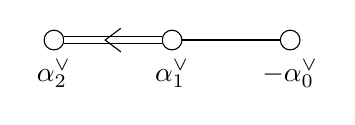
\begin{tikzpicture}[scale=1, baseline=-3pt, circ/.style={draw, circle, inner sep=2pt, minimum size=2.5mm}]
        \node[circ, label=below:$\alpha^\vee_2$] (0) at (0,0) {}; 
        \node[circ, label=below:$\alpha^\vee_1$] (1) at (1.5,0) {}; 
        \node[circ, label=below:$-\alpha^\vee_0$] (2) at (3,0) {}; 
        \draw (1)--(2);
        \draw[double, double distance=2pt] (0) -- (1);
        \draw (0.85,0.15) -- (0.65,0) -- (0.85,-0.15);% Arrow
    \end{tikzpicture}
\end{center}
Thus $G_2(F)$ has $3$ classes of maximal parahoric subgroups $K_0$, $K_1$, $K_2$ corresponding to the subsets of affine simple roots $J_0=\{\alpha^\vee_1,\alpha^\vee_2\}, J_1=\{-\alpha^\vee_0,\alpha^\vee_2\}$ and $J_2=\{-\alpha^\vee_0,\alpha^\vee_1\}$ and with reductive types $G_2$, $A_1\times \tilde{A}_1$ and $A_2$, respectively. We now compute these parahoric restrictions for all representations $\pi(us,\phi)$ of $G=G_2(F)$, where $u$ is a subregular unipotent element of $G_2(\CC)$, labelled by $G_2(a_1)$. This is an interesting case since $u$ is a distinguished unipotent element and $\Gamma_u=A_u\cong S_3$. There are $8$ such representations, given by 
$$\pi(G_2(a_1),1,\phi),\phi\in\{\mathbf{1},\varepsilon,r\},\quad\pi(G_2(a_1),g_2,\phi),\phi\in\{\mathbf{1},\varepsilon\},\quad\pi(G_2(a_1),g_3,\phi),\phi\in\{\mathbf{1},\theta,\theta^2\}.$$
Lusztig's arithmetic-geometric correspondence directly implies that $4$ of them are unipotent supercuspidal representations of $G_2(F)$ given by 
\begin{align*}
    \pi(G_2(a_1),1,\epsilon)=\cInd_{K_0}^{G}G_2[1],\quad&\pi(G_2(a_1),g_2,\epsilon)=\cInd_{K_0}^{G}G_2[-1]\quad\text{and}\\
    \quad\pi(G_2(a_1),g_3,\theta^k)=&\cInd_{K_0}^{G}G_2[\theta^k], k=1,2,
\end{align*}
while the remaining $4$ are Iwahori-spherical. 
For the supercuspidal representations, their restrictions can be easily computed. By Frobenius reciprocity, their parahoric restrictions to $K_0$ are irreducible, while the remaining parahoric restrictions are $0$.

To compute parahoric restriction of Iwahori-spherical representations, we recall that we work inside \textit{complex} Weyl group $W$ and consequently $s_0$ is as a short reflection along $\alpha_0$, while $s^0$ is the long reflection along $\alpha^0$. The unipotent element $u\in G^\vee=G_2(\CC)$ is subregular, so by Springer theory
$$H^*(\mathcal{B}^u)^\mathbf{1}=H^0(\mathcal{B}^u)^\mathbf{1}+H^2(\mathcal{B}^u)^\mathbf{1}=\phi_{1,0}+\phi_{2,1},\quad\text{and}\quad H^*(\mathcal{B}^u)^r=H^0(\mathcal{B}^u)^r+H^2(\mathcal{B}^u)^r=\phi_{1,3}'$$
as $W$-modules. On the other hand, $u$ is a regular unipotent element in $G^\vee_{g_2}=\GL_2(\CC)$ and $G^\vee_{g_3}=\SL_3(\CC)$, so $H^0(\mathcal{B}_{g_2}^u)$ and $H^0(\mathcal{B}_{g_3}^u)$ afford the trivial representations of $W_{g_2}=\langle s^0,s_1\rangle$ and $W_{g_3}=\langle s^0,s_2\rangle$ respectively, and
$$\Ind_{W_{g_2}}^W\mathbf{1}=\phi_{1,0}+\phi_{1,3}''\quad\text{and}\quad\Ind_{W_{g_3}}^W\mathbf{1}=\phi_{1,0}+\phi_{2,2}.$$
To obtain the parahoric restrictions to $K_0$, we note that all characters $\chi_t^{J_0}$ are trivial so it remains to twist by $\varepsilon=\phi_{1,6}$ (swapping $\phi_{1,0}\leftrightarrow\phi_{1,6}$ and $\phi_{1,3}'\leftrightarrow\phi_{1,3}''$) and then by the outer automorphism of $W$ exchanging short and long roots (swapping $\phi_{1,3}'\leftrightarrow\phi_{1,3}''$ only). 

To compute the parahoric restrictions with respect to $K_1$ and $K_2$ in Table \ref{tbl:G2_restriction} we compute the remaining characters $\chi_t^J$. Using their properties above, one can check that all characters are trivial except for the pairs $(s,J)=(g_3,J_2)$ and $(s,J)=(g_2,J_1)$. When the characters are trivial, Lemma \ref{lem:mackey_restriction} and Alvis' tables immediately yield the results. The last two cases must be dealt with separately.
\begin{itemize}
    \item \textbf{Restriction of $\pi(G_2(a_1),g_3,1)$ to $K_{J_2}$.} In this case, $W_{J_2}=\langle s_0,s_1\rangle$ (where $s_0$ is the reflection along the highest short root) and $W_{g_3}=\langle s^0,s_2\rangle$ (where $s^0$ is the reflection along the highest root). Then $W_{g_3}\backslash W/W_{J_2}=\{1\}$, $W_{J_2,g_3}\cong C_3$ and $\chi_{g_3}^{J_2}$ is a primitive character. Thus, 
    $$\Ind_{W_{J_2,g_3}}^{W_{J_2}}\chi_{g_3}^{J_2}=r.$$ 
    \item \textbf{Restriction of $\pi(G_2(a_1),g_2,1)$ to $K_{J_1}$.} In this case, $W_{J_1}=\langle s_0,s_2\rangle$ and $W_{g_2}=\langle s^0,s_1\rangle$, so $W_{g_2}\backslash W/W_{J_1}=\{1,w\}$ has two elements. Then, $W_{J_1,g_2}\cong C_2$ with $\chi_{g_2}^{J_1}$ non-trivial character and $W_{J_1,g_2^w}=W_{J_1}$ with $\chi_{g_2^w}^{J_1}$ the trivial character. Thus,
    $$\Ind_{W_{J_1,g_2}}^{W_{J_1}}\chi_{g_2}^{J_1}+\Ind_{W_{J_1,g_2^w}}^{W_{J_1}}\chi_{g_2^w}^{J_1}=\varepsilon\boxtimes\mathbf{1}+\mathbf{1}\boxtimes\varepsilon+\mathbf{1}\boxtimes\mathbf{1}.$$ 
\end{itemize}

\iffalse
\begin{figure}[ht]
    \centering
    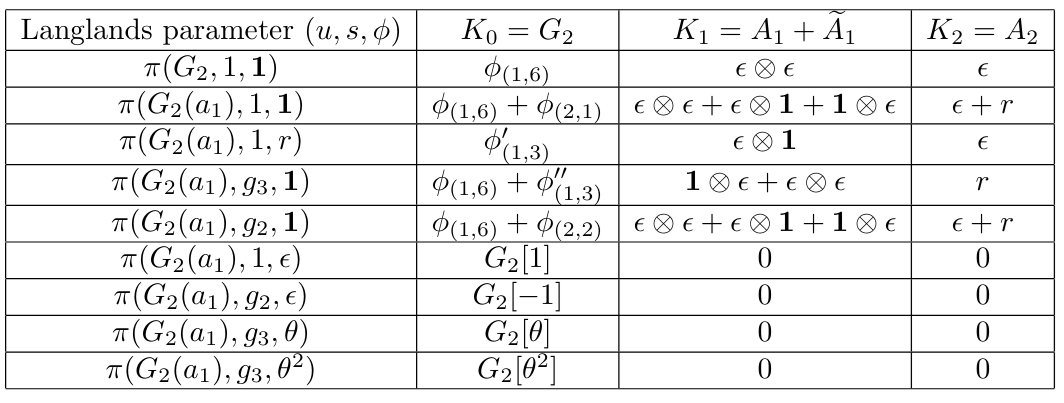
\includegraphics[scale=0.7]{subregular_element.png}
    \caption{Restrictions of $G_2$-representations $\pi(G_2(a_1),s,\phi)$}
    \label{tbl:G2_restriction_deleted}
\end{figure}
\fi

Twisting by the sign character yields the desired result. The proof of Conjecture \ref{conj:main} is now just a matter of putting all the pieces together. The parahoric restrictions of the virtual characters $\Pi(u,s,h)$ can be computed by linearity from the parahoric restrictions of the representations $\pi(u,s,\phi)$, which are given in Table \ref{tbl:G2_restriction}. 
\begin{table}[ht]
    \centering
    \begin{tabular}{|c|c|c|c|}
        \hline
        & $K_0\longrightarrow G_2$ & $K_1\longrightarrow A_1\times\tilde{A}_1$ & $K_2\longrightarrow A_2$ \\\hline
        $\Pi(G_2,1,1)$ & $\phi_{1,6}$ & $\epsilon\boxtimes\epsilon$ & $\epsilon$ \\\hline
        $\Pi(G_2(a_1),1,1)$ & $\phi_{2,1}+G_2[1]+2\phi_{1,3}'+\phi_{1,6}$ & $\mathbf{1}\boxtimes\epsilon+3\epsilon\boxtimes\mathbf{1}+\epsilon\boxtimes\epsilon$ & $3\epsilon+r$ \\\hline
        $\Pi(G_2(a_1),1,g_2)$ & $\phi_{2,1}-G_2[1]+\phi_{1,6}$ & $\mathbf{1}\boxtimes\epsilon+\epsilon\boxtimes\mathbf{1}+\epsilon\boxtimes\epsilon$ & $\epsilon+r$ \\\hline
        $\Pi(G_2(a_1),g_2,1)$ & $\phi_{2,1}+\phi_{2,2}+G_2[-1]+\phi_{1,6}$ & $\mathbf{1}\boxtimes\epsilon+\epsilon\boxtimes\mathbf{1}+\epsilon\boxtimes\epsilon$ & $\epsilon+r$ \\\hline
        $\Pi(G_2(a_1),1,g_3)$ & $\phi_{2,1}+G_2[1]-\phi_{1,3}'+\phi_{1,6}$ & $\mathbf{1}\boxtimes\epsilon+\epsilon\boxtimes\epsilon$ & $r$ \\\hline
        $\Pi(G_2(a_1),g_3,1)$ & $\phi_{1,3}''+G_2[\theta]+G_2[\theta^2]+\phi_{1,6}$ & $\mathbf{1}\boxtimes\epsilon+\epsilon\boxtimes\epsilon$ & $r$ \\\hline
        $\Pi(G_2(a_1),g_2,g_2)$ & $\phi_{2,1}+\phi_{2,2}-G_2[-1]+\phi_{1,6}$ & $\mathbf{1}\boxtimes\epsilon+\epsilon\boxtimes\mathbf{1}+\epsilon\boxtimes\epsilon$ & $\epsilon+r$ \\\hline
        $\Pi(G_2(a_1),g_3,g_3)$ & $\phi_{1,3}''+\theta G_2[\theta]+\theta^2 G_2[\theta^2]+\phi_{1,6}$ & $\mathbf{1}\boxtimes\epsilon+\epsilon\boxtimes\epsilon$ & $r$ \\\hline
        $\Pi(G_2(a_1),g_3,g_3^{-1})$ & $\phi_{1,3}''+\theta^2 G_2[\theta]+\theta G_2[\theta^2]+\phi_{1,6}$ & $\mathbf{1}\boxtimes\epsilon+\epsilon\boxtimes\epsilon$ & $r$ \\\hline
    \end{tabular}
    \caption{Restrictions of $G_2$-representations $\pi(G_2(a_1),s,\phi)$}
    \label{tbl:G2_restriction}
\end{table}

Finally, Lusztig's nonabelian Fourier transform acts trivially on every representation, except for the $G_2(\FF_q)$ family 
$$\{\phi_{2,1},\phi_{1,3}',G_2[1],\phi_{2,2},G_2[-1],\phi_{1,3}'',G_2[\theta],G_2[\theta^2]\},$$
where the action is given by the $8\times 8$ matrix
\begin{equation*}
    \begin{pmatrix}
        \frac{1}{6} & \frac{1}{3} & \frac{1}{6} & \frac{1}{2} & \frac{1}{2} & \frac{1}{3} & \frac{1}{3} & \frac{1}{3} &\\
        \frac{1}{3} & \frac{2}{3} & \frac{1}{3} & 0 & 0 & -\frac{1}{3} & -\frac{1}{3} & -\frac{1}{3} \\
        \frac{1}{6} & \frac{1}{3} & \frac{1}{6} & -\frac{1}{2} & -\frac{1}{2} & \frac{1}{3} & \frac{1}{3} & \frac{1}{3} &\\
        \frac{1}{2} & 0 & -\frac{1}{2} & \frac{1}{2} & -\frac{1}{2} & 0 & 0 & 0\\
        \frac{1}{2} & 0 & -\frac{1}{2} & -\frac{1}{2} & \frac{1}{2} & 0 & 0 & 0\\
        \frac{1}{3} & -\frac{1}{3} & \frac{1}{3} & 0 & 0 & \frac{2}{3} & -\frac{1}{3} & -\frac{1}{3} \\
        \frac{1}{3} & -\frac{1}{3} & \frac{1}{3} & 0 & 0 & -\frac{1}{3} & \frac{2}{3} & -\frac{1}{3} \\
        \frac{1}{3} & -\frac{1}{3} & \frac{1}{3} & 0 & 0 & -\frac{1}{3} & -\frac{1}{3} & \frac{2}{3} 
    \end{pmatrix}
\end{equation*}
It is now a routine calculation to see that the square in Conjecture \ref{conj:main} commutes.